\chapter{Измерение момента инерции тестового маховика}\label{app:A}

Измеряют геометрические размеры маховика $D_1,D_2,D_3,L_1,L_2$. Чертёж маховика приведён на рисунке~\cref{fig:flywheel-sketch}.




\begin{figure}[h]
	\centering
	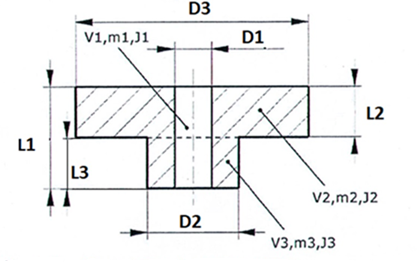
\includegraphics[width=.9\linewidth]{images/flywheel}
	\caption{Эскиз маховика}
	\label{fig:flywheel-sketch}
	\captionsetup{justification=centering}
	\vspace{2mm}
	\small
	\begin{minipage}{.92\linewidth}
		\textit{Обозначения (для расчётов):}
		\(V_1,m_1,J_1\) — объём, масса и момент инерции цилиндра;
		\(V_2,m_2,J_2\) — объём, масса и момент инерции большого диска;
		\(V_3,m_3,J_3\) — объём, масса и момент инерции малого диска.
	\end{minipage}
\end{figure}

Измерения выполняют штангенциркулем ШЦЦ-I-125-0,01
с абсолютной погрешностью \(\pm\SI{0.03}{\milli\meter}\).

\begin{table}[h]
	\centering
	\begin{threeparttable}
		\caption{Результаты измерений геометрических размеров}
		\label{tab:geom}
		\begin{tabular}{@{}lll@{}}
			\toprule
			Обозначение & Значение & Комментарий \\
			\midrule
			\(D_1\) & \SI{11.01}{\milli\meter} & диаметр вала \\
			\(D_2\) & \SI{69.03}{\milli\meter} & диаметр большого диска \\
			\(D_3\) & \SI{26.98}{\milli\meter} & диаметр малого диска \\
			\(L_1\) & \SI{30.04}{\milli\meter} & ширина большого диска \\
			\(L_2\) & \SI{15.08}{\milli\meter} & ширина малого диска \\
			\(L_3\) & \SI{14.96}{\milli\meter} & длина втулки/цилиндра \\
			\bottomrule
		\end{tabular}
	\end{threeparttable}
\end{table}


Измеряют массу маховика взвешиванием на весах EK-12Ki с пределом допускаемой погрешности \SI{\pm 3}{\gram}. масса маховика составляет $\SI{0,488}{\kilogram}$. 

Рассчитывают объём маховика как сумму объёмов составных частей:
\begin{equation}
	 V = V_2 + V_3 - V_1
\end{equation}

Объём одной составной части определяют как:
\begin{equation}
	V_i = \pi \cdot r_i^2 \cdot h_i
\end{equation}
где \(r_i\)--- радиус диска составной части маховика, \(h_i\)"--- высота составной части маховика.

\begin{equation}
 	\begin{aligned}
 		V_1 &= \pi r_1^2 h_1 = 2860 \,\text{мм}^3 = 2.860 \cdot 10^{-6}\,\text{м}^3, \\
 		V_2 &= \pi r_2^2 h_2 = 55972 \,\text{мм}^3 = 5.597 \cdot 10^{-5}\,\text{м}^3, \\
 		V_3 &= \pi r_3^2 h_3 = 8621 \,\text{мм}^3 = 8.552 \cdot 10^{-6}\,\text{м}^3, \\
 		V   &= 6.173 \cdot 10^{-5}\,\text{м}^3.
 	\end{aligned}
\end{equation}

Определяют погрешность измерения объёма:

\begin{equation}
	\begin{aligned}
		\Delta V_i &= V_i \sqrt{
			\left( \frac{\partial \ln(V_i)}{\partial r_i}\Delta r \right)^2 +
			\left( \frac{\partial \ln(V_i)}{\partial h_i}\Delta h \right)^2 }
		= V_i \sqrt{\left(\tfrac{2}{r_i}\Delta r\right)^2 + \left(\tfrac{1}{h_i}\Delta h\right)^2 } \\[1ex]
		\Delta V_1 &= 2860 \sqrt{ \left(\tfrac{2}{5.5}\cdot 0.03\right)^2 + \left(\tfrac{1}{30.04}\cdot 0.03\right)^2 }
		= 3.13 \cdot 10^{-8}\,\text{м}^3 \\[1ex]
		\Delta V_2 &= 55972 \sqrt{ \left(\tfrac{2}{34.515}\cdot 0.03\right)^2 + \left(\tfrac{1}{14.96}\cdot 0.03\right)^2 }
		= 1.48 \cdot 10^{-7}\,\text{м}^3 \\[1ex]
		\Delta V_3 &= 8621 \sqrt{ \left(\tfrac{2}{13.49}\cdot 0.03\right)^2 + \left(\tfrac{1}{15.08}\cdot 0.03\right)^2 }
		= 4.20 \cdot 10^{-8}\,\text{м}^3 \\[1ex]
		\Delta V   &= \sqrt{(\Delta V_1)^2 + (\Delta V_2)^2 + (\Delta V_3)^2}
		= 1.59 \cdot 10^{-7}\,\text{м}^3
	\end{aligned}
\end{equation}



Рассчитывают плотность материала маховика по формуле:
\begin{equation}
\rho = \frac{m}{V} = \frac{0.488}{6.173 \cdot 10^{-5}}
= 7905 \,\si{\kilo\gram\per\cubic\meter}
\end{equation}

Находят погрешность измерения плотности $\rho$:

\begin{equation}
	\begin{alignedat}{2}
		\Delta \rho &= 
		\sqrt{\left( \frac{\partial \ln(\rho)}{\partial m} \, \Delta m \right)^{2} +
			\left( \frac{\partial \ln(\rho)}{\partial V} \, \Delta V \right)^{2}}, \\[1ex]
		\Delta \rho &= 7905 \cdot 
		\sqrt{(0.003)^{2} + (1.59 \cdot 10^{-7})^{2}}
		= 2.37 \cdot 10^{-5}\,\frac{\text{кг}}{\text{м}^3}
	\end{alignedat}
\end{equation}

Определяют массу составных частей маховика по формуле:

\begin{equation}
	\begin{alignedat}{1}
		m_i &= V_i \cdot \rho, \\[1ex]
		m_1 &= 2.860 \cdot 10^{-6} \cdot 7905 = 0.0226 \,\text{кг}, \\[1ex]
		m_2 &= 5.597 \cdot 10^{-5} \cdot 7905 = 0.4424 \,\text{кг}, \\[1ex]
		m_3 &= 8.552 \cdot 10^{-6} \cdot 7905 = 0.0677 \,\text{кг}.
	\end{alignedat}
\end{equation}

Определяют погрешность определения массы составных частей:

\begin{equation}
	\begin{aligned}
		\Delta m_i &= m_i \sqrt{
			\left( \frac{\partial \ln(m_i)}{\partial V_i} \Delta V_i \right)^{2} +
			\left( \frac{\partial \ln(m_i)}{\partial \rho} \Delta \rho \right)^{2}}, \\[1ex]
		\Delta m_1 &= 0.0226 \cdot \sqrt{(3.13 \cdot 10^{-8})^{2} + (2.37 \cdot 10^{-5})^{2}}
		= 5.36 \cdot 10^{-7}\,\text{кг}, \\[1ex]
		\Delta m_2 &= 0.4424 \cdot \sqrt{(1.48 \cdot 10^{-7})^{2} + (2.37 \cdot 10^{-5})^{2}}
		= 1.04 \cdot 10^{-5}\,\text{кг}, \\[1ex]
		\Delta m_3 &= 0.0677 \cdot \sqrt{(1.59 \cdot 10^{-7})^{2} + (2.37 \cdot 10^{-5})^{2}}
		= 1.61 \cdot 10^{-6}\,\text{кг}.
	\end{aligned}
\end{equation}

Определяют момент инерции составных частей маховика по формуле:
\begin{equation}
	\begin{aligned}
		J_i &= \frac{m_i}{2} \, r_i^{2}, \\[1ex]
		J_1 &= \frac{m_1}{2} \, r_1^{2} = 3.42 \cdot 10^{-7}\,\text{кг}\cdot\text{м}^2, \\[1ex]
		J_2 &= \frac{m_2}{2} \, r_2^{2} = 2.63 \cdot 10^{-4}\,\text{кг}\cdot\text{м}^2, \\[1ex]
		J_3 &= \frac{m_3}{2} \, r_3^{2} = 6.20 \cdot 10^{-6}\,\text{кг}\cdot\text{м}^2.
	\end{aligned}
\end{equation}

Определяют погрешность измерения момента инерции составных частей маховика по формуле:

\begin{equation}
	\begin{aligned}
		J_i &= J_i \sqrt{
			\left( \frac{\partial \ln(J_i)}{\partial m_i}\,\Delta m_i \right)^{2} +
			\left( \frac{\partial \ln(J_i)}{\partial r_i}\,\Delta r \right)^{2}}, \\[1ex]
		\Delta J_1 &= J_1 \sqrt{
			\left( \frac{\partial \ln(J_1)}{\partial m_1}\,\Delta m_1 \right)^{2} +
			\left( \frac{\partial \ln(J_1)}{\partial r_1}\,\Delta r \right)^{2}}
		= 3.73 \cdot 10^{-9}\,\text{кг}\cdot\text{м}^2, \\[1ex]
		\Delta J_2 &= J_2 \sqrt{
			\left( \frac{\partial \ln(J_2)}{\partial m_2}\,\Delta m_2 \right)^{2} +
			\left( \frac{\partial \ln(J_2)}{\partial r_2}\,\Delta r \right)^{2}}
		= 4.58 \cdot 10^{-7}\,\text{кг}\cdot\text{м}^2, \\[1ex]
		\Delta J_3 &= J_3 \sqrt{
			\left( \frac{\partial \ln(J_3)}{\partial m_3}\,\Delta m_3 \right)^{2} +
			\left( \frac{\partial \ln(J_3)}{\partial r_3}\,\Delta r \right)^{2}}
		= 2.75 \cdot 10^{-8}\,\text{кг}\cdot\text{м}^2.
	\end{aligned}
\end{equation}

Итоговая погрешность составляет:
\begin{equation}
	\Delta J = \sqrt{ (\Delta J_1)^2 + (\Delta J_2)^2 + (\Delta J_3)^2 }
	= 4.58 \cdot 10^{-7}\,\text{кг}\cdot\text{м}^2
\end{equation}

 

\clearpage
\refstepcounter{chapter}


